\section{Component Class Reference}
\label{classComponent}\index{Component@{Component}}
{\tt \#include $<$component.h$>$}

Inheritance diagram for Component:\nopagebreak
\begin{figure}[H]
\begin{center}
\leavevmode

\includegraphics[width=400pt]{classComponent__inherit__graph}
\end{center}
\end{figure}
Collaboration diagram for Component:\nopagebreak
\begin{figure}[H]
\begin{center}
\leavevmode
\includegraphics[height=400pt]{classComponent__coll__graph}
\end{center}
\end{figure}
\subsection*{Public Member Functions}
\begin{CompactItemize}
\item 
{\bf Component} ()
\item 
{\bf Component} (int lpId)
\item 
{\bf $\sim$Component} ()
\item 
void {\bf setComponentId} (int id)
\item 
void {\bf addInputLink} ({\bf Link} $\ast$l)
\item 
void {\bf addOutputLink} ({\bf Link} $\ast$l)
\item 
int {\bf myId} ()
\end{CompactItemize}
\subsection*{Public Attributes}
\begin{CompactItemize}
\item 
std::vector$<$ {\bf Link} $\ast$ $>$ {\bf inLinks}
\item 
std::vector$<$ {\bf Link} $\ast$ $>$ {\bf outLinks}
\end{CompactItemize}
\subsection*{Private Attributes}
\begin{CompactItemize}
\item 
int {\bf componentId}
\end{CompactItemize}


\subsection{Detailed Description}


Definition at line 11 of file component.h.

\subsection{Constructor \& Destructor Documentation}
\index{Component@{Component}!Component@{Component}}
\index{Component@{Component}!Component@{Component}}
\subsubsection[{Component}]{\setlength{\rightskip}{0pt plus 5cm}Component::Component ()}\label{classComponent_8775db6d1a2c1afc2e77cd3c8f39da6f}




Definition at line 10 of file component.cc.

References Simulator::registerComponent().\index{Component@{Component}!Component@{Component}}
\index{Component@{Component}!Component@{Component}}
\subsubsection[{Component}]{\setlength{\rightskip}{0pt plus 5cm}Component::Component (int {\em lpId})}\label{classComponent_52f5a349d8ed4bd7efd4c8ee381a0ed8}




Definition at line 15 of file component.cc.

References Simulator::registerComponent().\index{Component@{Component}!$\sim$Component@{$\sim$Component}}
\index{$\sim$Component@{$\sim$Component}!Component@{Component}}
\subsubsection[{$\sim$Component}]{\setlength{\rightskip}{0pt plus 5cm}Component::$\sim$Component ()}\label{classComponent_b8378fa275af98e568a7e91d33d867af}




Definition at line 5 of file component.cc.

\subsection{Member Function Documentation}
\index{Component@{Component}!addInputLink@{addInputLink}}
\index{addInputLink@{addInputLink}!Component@{Component}}
\subsubsection[{addInputLink}]{\setlength{\rightskip}{0pt plus 5cm}void Component::addInputLink ({\bf Link} $\ast$ {\em l})}\label{classComponent_9c7c91fe01f0d204cbc79b597d8236fe}




Definition at line 25 of file component.cc.

References inLinks.\index{Component@{Component}!addOutputLink@{addOutputLink}}
\index{addOutputLink@{addOutputLink}!Component@{Component}}
\subsubsection[{addOutputLink}]{\setlength{\rightskip}{0pt plus 5cm}void Component::addOutputLink ({\bf Link} $\ast$ {\em l})}\label{classComponent_aed97b38bbc44deddf329aa473e23b25}




Definition at line 30 of file component.cc.

References outLinks.

Referenced by Link::Link().

Here is the caller graph for this function:\nopagebreak
\begin{figure}[H]
\begin{center}
\leavevmode
\includegraphics[width=137pt]{classComponent_aed97b38bbc44deddf329aa473e23b25_icgraph}
\end{center}
\end{figure}
\index{Component@{Component}!myId@{myId}}
\index{myId@{myId}!Component@{Component}}
\subsubsection[{myId}]{\setlength{\rightskip}{0pt plus 5cm}int Component::myId ()\hspace{0.3cm}{\tt  [inline]}}\label{classComponent_af44955457bc84fa39a346ee70db916f}




Definition at line 24 of file component.h.

References componentId.

Referenced by GenericRouterVct::init(), GenericRouterVcs::init(), GenericRouterNoVcs::init(), GenericRouterAdaptive::init(), NetworkComponent::NetworkComponent(), uncore\_\-t::setup(), NI::setup(), GenericTPGVcs::setup(), GenericTPG::setup(), GenericSink::setup(), GenericRPG::setup(), GenericLink::setup(), GenericInterfaceVcs::setup(), GenericInterface::setup(), and GenericFlatMc::setup().

Here is the caller graph for this function:\nopagebreak
\begin{figure}[H]
\begin{center}
\leavevmode
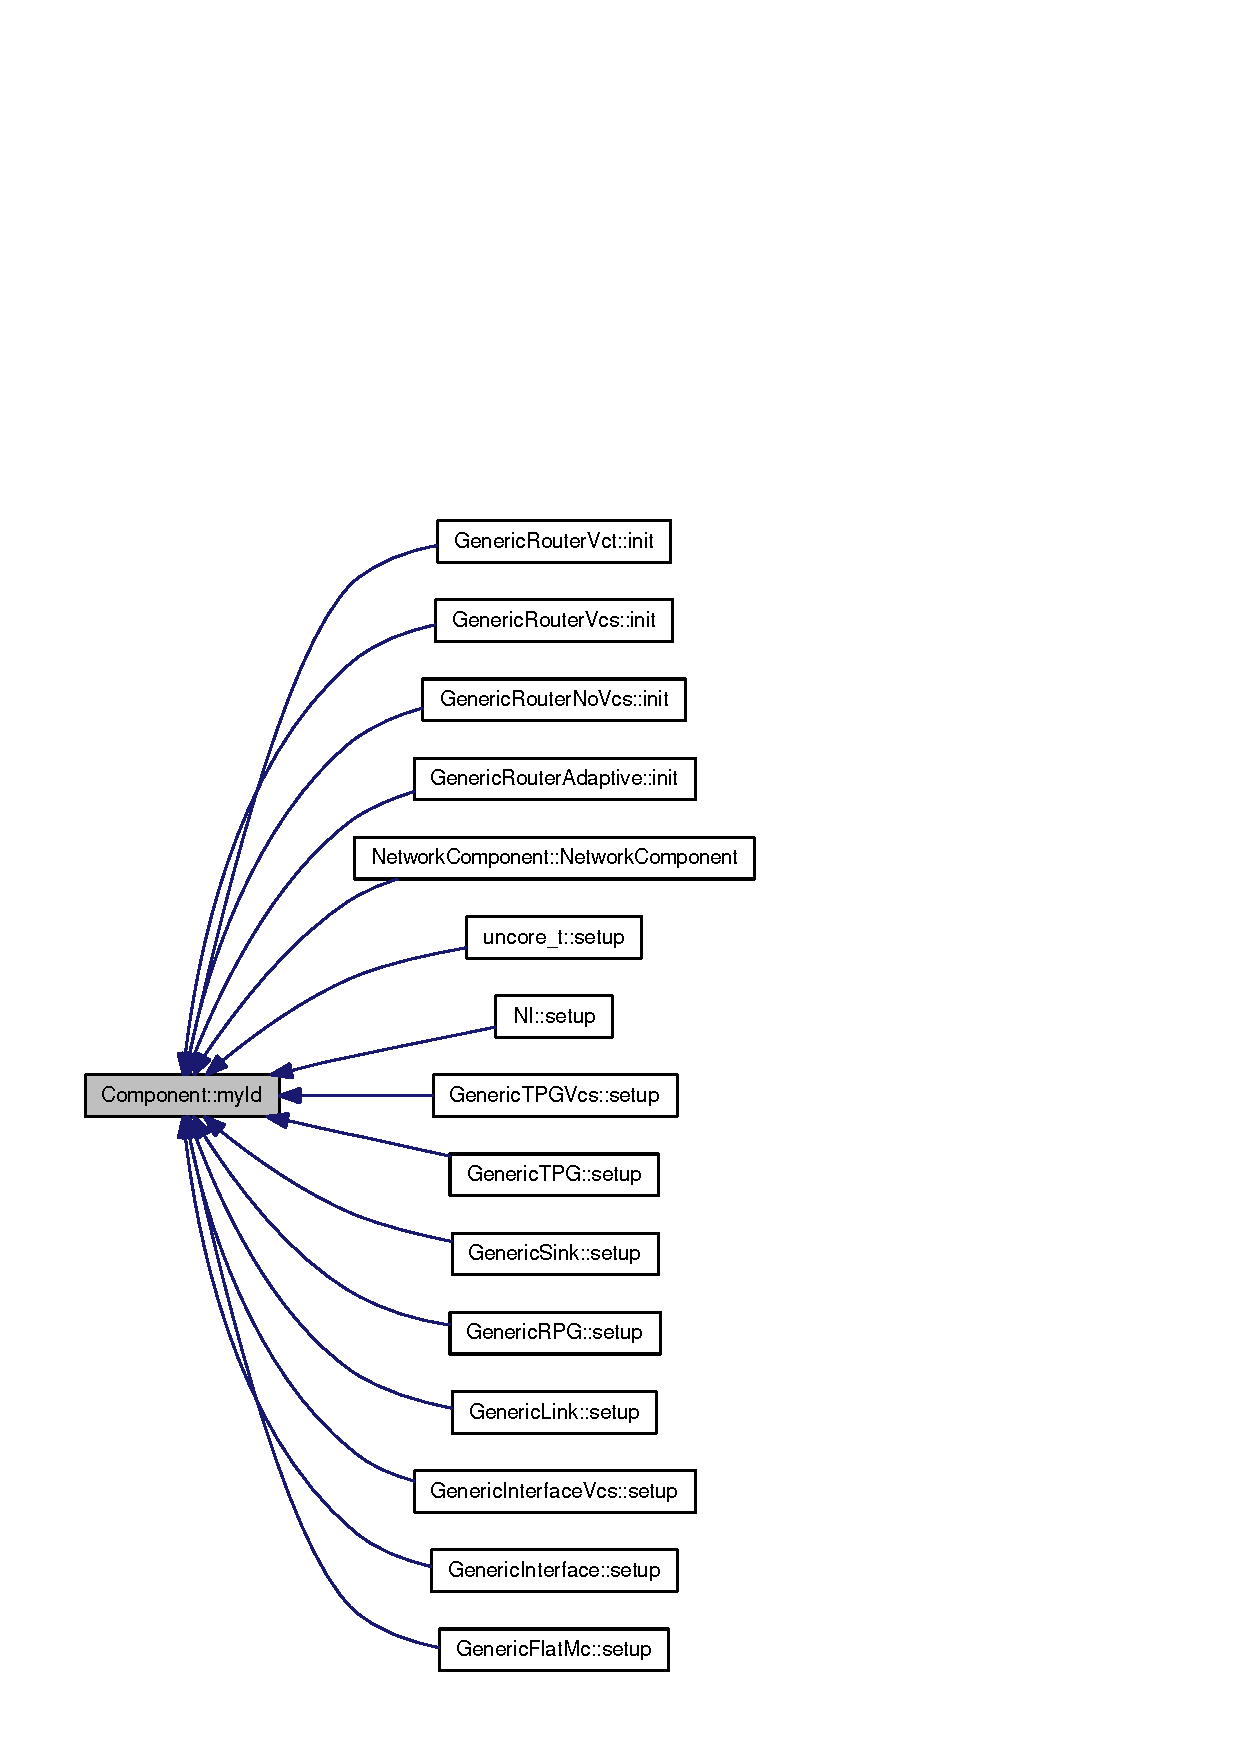
\includegraphics[width=183pt]{classComponent_af44955457bc84fa39a346ee70db916f_icgraph}
\end{center}
\end{figure}
\index{Component@{Component}!setComponentId@{setComponentId}}
\index{setComponentId@{setComponentId}!Component@{Component}}
\subsubsection[{setComponentId}]{\setlength{\rightskip}{0pt plus 5cm}void Component::setComponentId (int {\em id})}\label{classComponent_4a5ca86f7a92e163287c4aae16f6b4b2}




Definition at line 20 of file component.cc.

References componentId.

Referenced by Simulator::registerComponent().

Here is the caller graph for this function:\nopagebreak
\begin{figure}[H]
\begin{center}
\leavevmode
\includegraphics[width=264pt]{classComponent_4a5ca86f7a92e163287c4aae16f6b4b2_icgraph}
\end{center}
\end{figure}


\subsection{Member Data Documentation}
\index{Component@{Component}!componentId@{componentId}}
\index{componentId@{componentId}!Component@{Component}}
\subsubsection[{componentId}]{\setlength{\rightskip}{0pt plus 5cm}int {\bf Component::componentId}\hspace{0.3cm}{\tt  [private]}}\label{classComponent_64fb5507befa5f64a0d95003ea279c68}




Definition at line 14 of file component.h.

Referenced by myId(), and setComponentId().\index{Component@{Component}!inLinks@{inLinks}}
\index{inLinks@{inLinks}!Component@{Component}}
\subsubsection[{inLinks}]{\setlength{\rightskip}{0pt plus 5cm}std::vector$<${\bf Link}$\ast$$>$ {\bf Component::inLinks}}\label{classComponent_6c43e56775c15cfcc1c0e8a6cbc7c474}




Definition at line 16 of file component.h.

Referenced by addInputLink().\index{Component@{Component}!outLinks@{outLinks}}
\index{outLinks@{outLinks}!Component@{Component}}
\subsubsection[{outLinks}]{\setlength{\rightskip}{0pt plus 5cm}std::vector$<${\bf Link}$\ast$$>$ {\bf Component::outLinks}}\label{classComponent_4f715c718ecdb440f200e954b5d35b10}




Definition at line 17 of file component.h.

Referenced by addOutputLink().

The documentation for this class was generated from the following files:\begin{CompactItemize}
\item 
{\bf component.h}\item 
{\bf component.cc}\end{CompactItemize}
